%% Copyright (c) 2007 GeometryFactory (France).  All rights reserved.
%%
%% This file is part of CGAL (www.cgal.org).
%% You can redistribute it and/or modify it under the terms of the GNU
%% General Public License as published by the Free Software Foundation,
%% either version 3 of the License, or (at your option) any later version.
%%
%% Licensees holding a valid commercial license may use this file in
%% accordance with the commercial license agreement provided with the software.
%%
%% This file is provided AS IS with NO WARRANTY OF ANY KIND, INCLUDING THE
%% WARRANTY OF DESIGN, MERCHANTABILITY AND FITNESS FOR A PARTICULAR PURPOSE.
%%
%% 
%%
%% Author(s)     : Fernando Cacciola <fernando.cacciola@geometryfactory.com>

\begin{figure}[htbp]
\begin{ccTexOnly}
\begin{center}
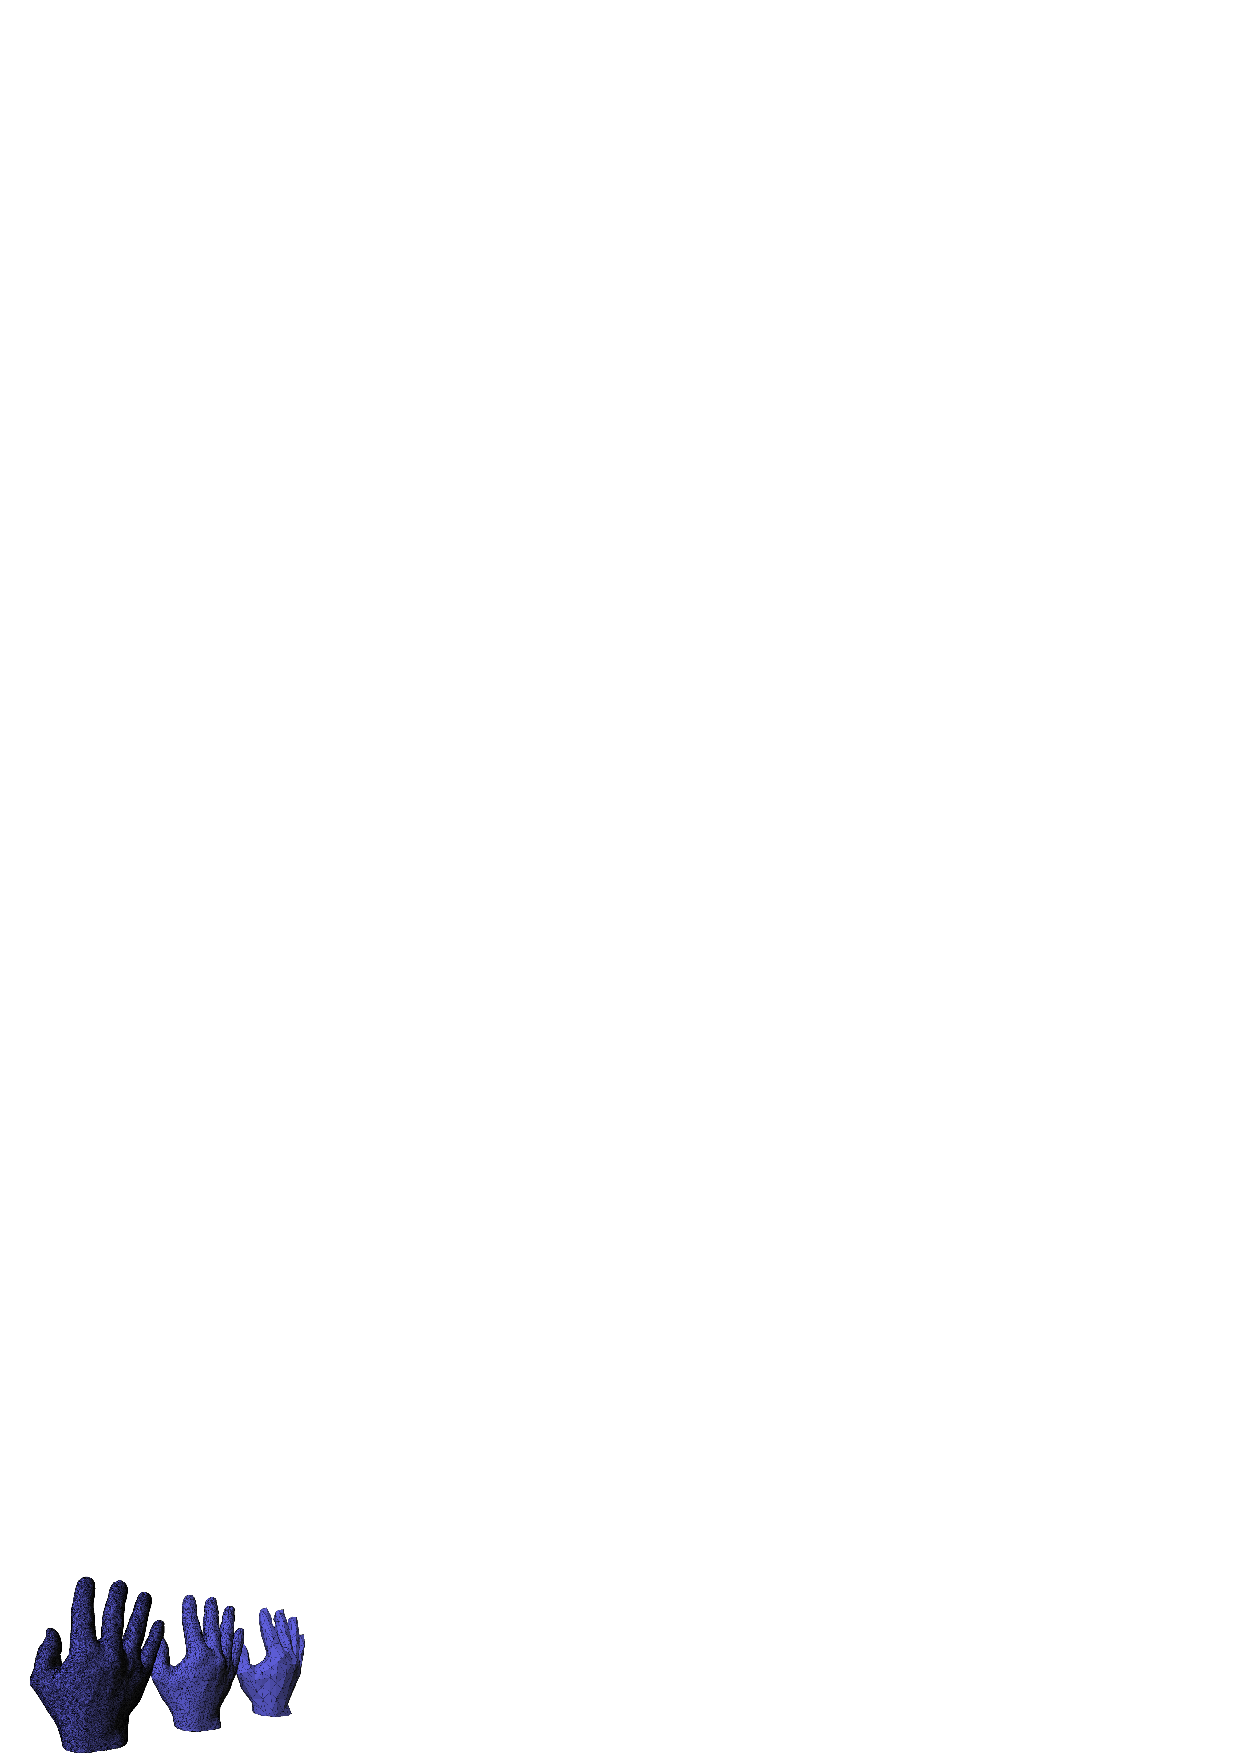
\includegraphics[width=17cm]{Surface_mesh_simplification/fig/Illustration-Simplification-ALL} % omit suffix .eps to support PS and PDF
\end{center}
\end{ccTexOnly}
\begin{ccHtmlOnly}
<TABLE CELLSPACING=40>
<TR>
<CENTER>
<IMG BORDER=0 SRC="./fig/Illustration-Simplification-ALL.jpg" ALIGN=middle ALT="Simplification illustration">
</CENTER>
</TR>
</TABLE>
\end{ccHtmlOnly}
\end{figure}
%% figures of simplified surfaces

\section{Introduction}
Surface mesh  simplification is the process of reducing the number of faces used in the surface while 
keeping the overall shape, volume and boundaries preserved as much as possible. 
It is the opposite of subdivision.

The algorithm presented here can simplify any {\em oriented 2-manifold surface},
with any number of connected components, with or without boundaries (border or holes) 
and handles (arbitrary genus), using a method known as {\em edge collapse}.
Roughly speaking, the method consists of iteratively replacing an edge with a single vertex, 
removing 2 triangles per collapse.


Edges are collapsed according to a priority given by a user-supplied {\em cost} function,
and the coordinates of the replacing vertex are determined by another user-supplied
{\em placement} function. The algorithm terminates when a user-supplied {\em stop predicate} 
is met, such as reaching the desired number of edges.

The algorithm implemented here is generic in the sense that it does not require the surface 
to be of a particular type. Instead, it defines the concept of a \ccc{EdgeCollapsableMesh},
which presents the surface as being a halfedge data structure, and any surface that 
is a model of that concept can be simplified.\
The concept is defined not in terms of a monolithic class, but in terms of a set 
of functions and traits, making it easy to adapt any concrete surface type, 
even if it is not a halfedge data structure at all.
In particular, the concept definition follows the design of the 
\ccAnchor{http://www.boost.org/libs/graph/doc/index.html}{ Boost Graph Library ({\sc Bgl})}
\cite{cgal:sll-bgl-02}.

The design is \ccAnchor{http://en.wikipedia.org/wiki/Policy-based_design}{{\em policy-based}}
(\path|http://en.wikipedia.org/wiki/Policy-based_design|),
meaning that you can customize some aspects of the process by passing a set of
{\em policy objects}. Each policy object specifies a particular aspect of the algorithm,
such as how edges are selected and where the replacement vertex is placed. All policies have 
a sensible default.
Furthermore, the API uses the so-called \ccc{named-parameters} technique which allows you
to pass only the relevant parameters, in any order, omitting those parameters whose
default is appropriate.

\section{Overview of the Simplification Process}

The free function that implements the simplification algorithm takes not only the surface
and the desired stop predicate but a number of additional parameters which control and
monitor the simplification process. This section briefly describes the process in order 
to set the background for the discussion of the parameters to the algorithm.

There are two slightly different "edge" collapse operations. One is known as
{\em edge-collapse} while the other is known as {\em halfedge-collapse}.
Given an edge 'e' joining vertices 'w' and 'v', the edge-collapse operation replaces
'e','w' and 'v' for a new vertex 'r', while the halfedge-collapse operation
pulls 'v' into 'w', dissapearing 'e' and leaving 'w' in place.
In both cases the operation removes the edge 'e' along with the 2 triangles 
adjacent to it.

This package uses the halfedge-collapse operation, which is implemented by removing,
additionally, 1 vertex ('v') and 2 edges, one per adjacent triangle.
It optionally moves the remaining vertex ('w') into a new position, 
called {\em placement}, in which case the net effect is the same as in
the edge-collapse operation.

%% figure of edge collapse

Naturally, the surface that results from an edge collapse deviates from the initial 
surface by some amount, and since the goal of simplification is to reduce the number 
of triangles while retaining the overall look of the surface as much as possible, 
it is necessary to measure such a deviation. Some methods attempt to measure the 
total deviation from the initial surface to the completely simplified surface, 
for example, by tracking an accumulated error while keeping a history of the simplification 
changes. Other methods, like the one implemented in this package, attempt to measure only
the {\em cost} of each individual edge collapse  (the local deviation introduced by
a single simplification step) and plan the entire process as a sequence of steps 
of increasing cost. 

Global error tracking methods produce highly accurate simplifications but take up a lot 
of additional space. Cost-driven methods, like the one in this package, produce slightly 
less accurate simplifications but take up much less additional space, even none in some cases.

The cost-driven method implemented in this package is mainly based on \cite{cgal:lt-fmeps-98,cgal:lt-ems-99}, with contributions from \cite{hddms-mo-93}, \cite{gh-ssqem-97}
and \cite{degn-tpec-98}.

The algorithm proceeds in two stages. In the first stage, called {\em collection stage}, 
an initial {\em collapse cost} is assigned to each and every edge in the surface.
Then in the second stage, called {\em collapsing stage}, edges are 
processed in order of increasing cost. Some processed edges are collapsed 
while some are just discarded. Collapsed edges are replaced by a vertex and the collapse 
cost of all the edges now incident on the replacement vertex is recalculated, affecting 
the order of the remaining unprocessed edges.

Not all edges selected for processing are collapsed. A processed edge can be discarded 
right away, without being collapsed, if it doesn't satisfy certain topological
and geometric conditions.

The algorithm presented in \cite{gh-ssqem-97} contracts (collapses) arbitrary vertex pairs and not 
only edges by considering certain vertex pairs as forming a pseudo-edge and proceeding to collapse
both edges and pseudo-edges in the same way as in \cite{cgal:lt-fmeps-98,cgal:lt-ems-99} ( 
which is the algorithm implemented here). However, contracting an arbitrary vertex-pair may result in a non-manifold surface, but the current state of this package can only deal with manifold surfaces, thus, it can only collapse edges. That is, this package cannot be used as a framework for vertex contraction.

\section{Cost Strategy}

The specific way in which the collapse cost and vertex placement is
calculated is called the {\em cost strategy}. The user can choose 
different strategies in the form of policies and related parameters,
passed to the algorithm.
 
The current version of the package provides a set of policies implementing
two strategies: the Lindstrom-Turk strategy, which is the default, and 
a strategy consisting of an edge-length cost with an optional
midpoint placement (much faster but less accurate).

%\begin{ccAdvanced}
\subsection{Lindstrom-Turk Cost and Placement Strategy\label{SurfaceMeshSimplification:LindstromTurkStrategy}}

The main characteristic of the strategy presented in
\cite{cgal:lt-fmeps-98,cgal:lt-ems-99} is that the simplified surface
is not compared at each step with the original surface (or the surface
at a previous step) so there is no need to keep extra information,
such as the original surface or a history of the local changes. Hence
the name {\em memoryless} simplification.

At each step, all remaining edges are potential candidates for 
collapsing and the one with the lowest cost is selected.

The cost of collapsing an edge is given by the position chosen for the
vertex that replaces it. 

The replacement vertex position is computed as
the solution to a system of 3 linearly-independent linear equality constraints.
Each constraint is obtained by minimizing a quadratic objective function
subject to the previously computed constraints.\\
There are several possible candidate constraints and each is considered in order of importance.
A candidate constraint might be {\em incompatible} with the previously accepted constraints,
in which case it is rejected and the next constraint is considered.\\
Once 3 constraints have been accepted, the system is solved for the vertex position.

The first constraints considered preserves the shape of the surface boundaries 
(in case the edge profile has boundary edges).
The next constraints preserve the total volume of the surface.
The next constraints, if needed, optimize the local changes in volume and boundary shape.
Lastly, if a constraint is still needed (because the ones previously computed were incompatible),
a third (and last) constraint is added to favor equilateral triangles over elongated triangles.

The cost is then a weighted sum of the shape, volume and boundary optimization terms, where the user specifies the unit {\em weighting unit factor} for each term.

The local changes are computed independently for each edge using only
the triangles currently adjacent to it at the time when the edge 
is about to be collapsed, that is, after all previous collapses.
Thus, the transitive path of minimal local changes yields at
the end a global change reasonably close to the absolute minimum.
%\end{ccAdvanced}

\subsection{Cost Strategy Policies}

The cost strategy used by the algorithm is selected by means of two policies: 
\ccc{GetPlacement} and \ccc{GetCost}. 

The \ccc{GetPlacement} policy is called to compute the new position
for the remaining vertex after the halfedge-collapse. It returns
an optional value, which can be absent, in which case the 
remaining vertex is kept in its place.

The \ccc{GetCost} policy is called to compute the cost
of collapsing an edge. This policy uses the placement to compute
the cost (which is an error measure) and determines the 
ordering of the edges.

The algorithm maintains an internal data structure (a mutable priority queue)
which allows each edge to be processed in increasing cost order. Such a data structure
requires some per-edge additional information, such as the edge's cost.
If the record of per-edge additional information occupies N bytes of storage,
simplifying a surface of 1 million edges (a normal size) requires 1 million times N bytes
of additional storage. Thus, to minimize the amount of additional memory required to
simplify a surface only the cost is attached to each edge and nothing else.

But this is a tradeoff: the cost of a collapse is a function of the placement
(the new position chosen for the remaining vertex) so before \ccc{GetCost}
is called for each and every edge, \ccc{GetPlacement} must also be called to obtain
the placement parameter to the cost function.
But that placement, which is a 3D Point, is not attached to each and every edge since
that would easily {\em triple} the additional storage requirement.

On the one hand, this dramatically saves on memory but on the other hand is
a processing waste because when an edge is effectively collapsed, \ccc{GetPlacement} 
must be called {\em again} to know were to move the remaining vertex.

Earlier prototypes shown that attaching the placement to the edge, thus avoiding one
redundant call to the placement function after the edge collapsed, has little 
impact on the total running time. This is because the cost of an each edge is not just
computed once but changes several times during the process so the placement function
must be called several times just as well. Caching the placement can only avoid the 
very last call, when the edge is collapsed, but not all the previous calls which
are needed because the placement (and cost) changes.

\section{API}

\subsection{API Overview}

Since the algorithm is free from robustness issues there is no need for exact predicates nor constructions and \ccc{Simple_cartesian<double>} can be used safely.
\footnote{In the current version, 3.3, the LindstromTurk policies are not implemented for homogeneous coordinates, so a cartesian kernel must be used.}

The simplification algorithm is implemented as the free template function 
\ccc{CGAL::Surface_mesh_simplification::edge_collapse}. The function has two mandatory and several optional parameters.

\subsubsection{Mandatory Parameters}

There are two main parameters to the algorithm: the surface to be simplified (in-place) and the stop predicate.

The surface to simplify must be a model of the \ccc{EdgeCollapsableMesh} concept. 
Many concrete surface types, such as \ccc{CGAL::Polyhedron_3} with only triangular faces,
become models of that concept via a technique known as 
{\em external adaptation}, which is described in \cite{cgal:sll-bgl-02}
and this {\sc Bgl} web page: \path|http://www.boost.org/libs/graph/doc/leda_conversion.html|

External adaptation is a way to add an interface to an 
object without coercing the type of the object (which happens when you adapt it by means 
of a wrapper). That is, the formal parameter to the \ccc{edge_collapse} function that 
implements the simplification is the concrete surface object itself, not an adaptor 
which delegates the functionality to the concrete type.

The stop predicate is called after each edge is selected for processing, {\em before} 
it is classified as collapsible or not (thus before it is collapsed). If the stop predicate 
returns \ccc{true} the algorithm terminates.

\subsubsection{Optional Named Parameters}

The notion of {\em named parameters} was also introduced in the {\sc Bgl}. You can read about it in \cite{cgal:sll-bgl-02} or the following site: \path|http://www.boost.org/libs/graph/doc/bgl_named_params.html|. Named parameters allow the user to specify only those parameters which are really needed, by name, making the parameter ordering unimportant. 

Say there is a function \ccc{f()} that takes 3 parameters called \ccc{name}, \ccc{age} and \ccc{gender}, and you have variables \ccc{n,a and g} to pass as parameters to that function. Without named parameters, you would call it like this: \ccc{f(n,a,g)}, but with named parameters, you call it like this: \ccc{f(name(n).age(a).gender(g))}.

That is, you give each parameter a name by wrapping it into a function whose name matches that of the parameter. The entire list of named parameters is really a composition of function calls separated by a dot ($.$). Thus, if the function takes a mix of mandatory and named parameters, you use a comma to separate the last non-named parameter from the first named parameters, like this:

\ccc{f(non_named_par0, non_named_pa1, name(n).age(a).gender(g)) }

When you use named parameters, the ordering is irrelevant, so this: \ccc{f(name(n).age(a).gender(g))} is equivalent to this:
\ccc{f(age(a).gender(g).name(n))}, and you can just omit any named parameter that has a default value.

\subsubsection{Sample Call}

\begin{ccExampleCode}
/*
surface                  : the surface to simplify
stop_predicate           : policy indicating when the simplification must finish 
vertex_index_map(vimap)  : property-map giving each vertex a unique integer index 
edge_index_map(eimap)    : property-map giving each edge a unique integer index 
edge_is_border_map(ebmap): property-map specifying whether an edge is a border edge or not 
get_cost(cf)             : function object computing the cost of a collapse 
get_placement(pf)        : function object computing the placement for the remaining vertex 
visitor(vis)             : function object tracking the simplification process 
*/
int r = edge_collapse(surface
                     ,stop_predicate
                     ,vertex_index_map(vimap)
                       .edge_index_map(eimap)
                       .edge_is_border_map(ebmap)
                       .get_cost(cf)
                       .get_placement(pf)
                       .visitor(vis)
                     );
\end{ccExampleCode}



\subsection{Examples}

\subsubsection{Example Using a Default Polyhedron}

The following example illustrates the simplest of the cases. It uses
an ordinary polyhedron and only one of the optional parameters.
The unspecified cost strategy defaults to Lindstrom-Turk.
\ccIncludeExampleCode{Surface_mesh_simplification/edge_collapse_polyhedron.cpp}

\subsubsection{Example Using an Enriched Polyhedron}

The following example is equivalent to the previous example but using an
enriched polyhedron whose halfedges support an \ccc{id} field to
store the edge index needed by the algorithm. It also shows how to
explicitly specify a cost strategy (other than the default)
and how to use a visitor object to track the simplification process.

\ccIncludeExampleCode{Surface_mesh_simplification/edge_collapse_enriched_polyhedron.cpp}

\subsubsection{Example with edges marked as non-removable}

The following example shows how to use the optional named parameter \ccc{edge_is_border_map} to prevent
edges from being removed even if they are not really borders.

\ccIncludeExampleCode{Surface_mesh_simplification/edge_collapse_constrained_polyhedron.cpp}

% +------------------------------------------------------------------------+
%%RefPage: end of main body, begin of sfsooter
% EOF
% +------------------------------------------------------------------------+


